\documentclass{article}
\usepackage{amsmath,amssymb,amsfonts}
\usepackage{algorithmic}
\usepackage{multicol}
\usepackage{graphicx}
\usepackage{array}
\graphicspath{ {./images/} }
\title{Assignment  for    Image  Recognition  and  Understanding\\
Assignment- 1}
\author{Chowdhury Md Intisar\\
ID -- m5212106
}

\begin{document}

\maketitle
\section{Color Image for Segmentation}


\begin{center}
\begin{table}
\begin{tabular}{c| c}
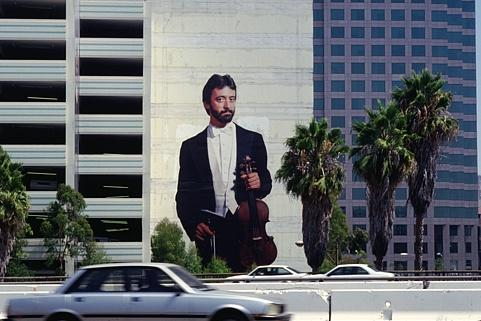
\includegraphics[scale = 0.3]{image1} & 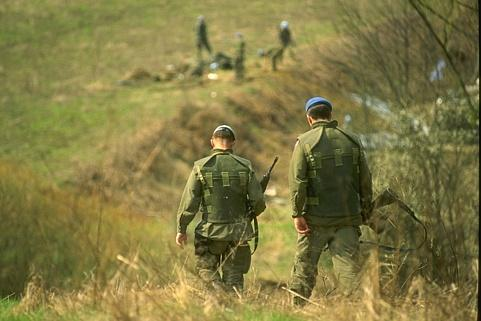
\includegraphics[scale = 0.3]{image2}\\
\\\hline\\
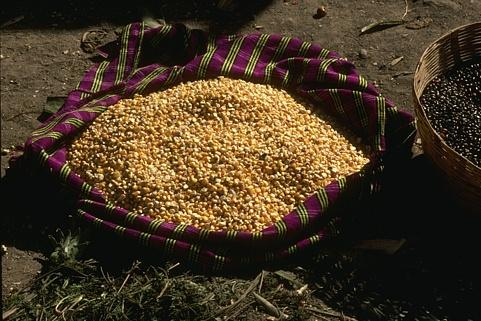
\includegraphics[scale = 0.3]{image3} & 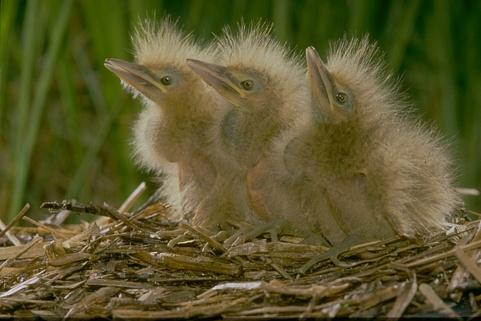
\includegraphics[scale = 0.3]{image4}\\
\end{tabular}
\caption{Input images for Segmentation.}
\label{table:1}
\end{table}
\end{center}


\section{Ground Truth segmentation image for comparison}


\begin{center}
\begin{table}
\begin{tabular}{c| c}
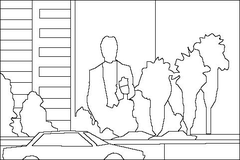
\includegraphics[scale = 0.7]{edge_1} & 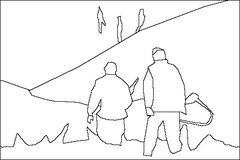
\includegraphics[scale = 0.7]{edge_2}\\
\\\hline\\
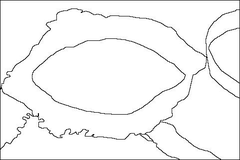
\includegraphics[scale = 0.7]{edge_3} & 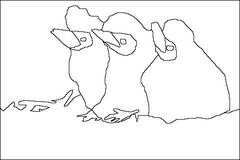
\includegraphics[scale = 0.7]{edge_4}\\
\end{tabular}
\caption{The Ground truth segmented images used for comparison.}
\label{table:2}
\end{table}
\end{center}


\begin{center}
\begin{table}
\begin{tabular}{c| c}
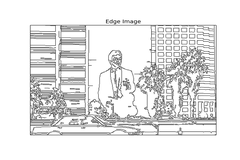
\includegraphics[scale = 0.7]{canny_1} & 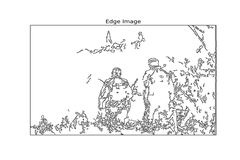
\includegraphics[scale = 0.7]{canny_2}\\
\\\hline\\
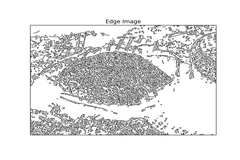
\includegraphics[scale = 0.7]{canny_3} & 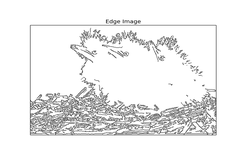
\includegraphics[scale = 0.7]{canny_4}\\
\end{tabular}
\caption{Output by color gradient segmentation. (Gradient method based on Canny).}
\label{table:3}
\end{table}
\end{center}



\begin{center}
\begin{table}
\begin{tabular}{c| c}
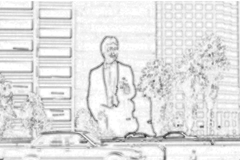
\includegraphics[scale = 0.7]{log_1} & 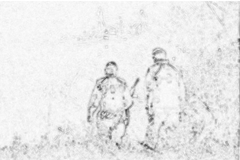
\includegraphics[scale = 0.7]{log_2}\\
\\\hline\\
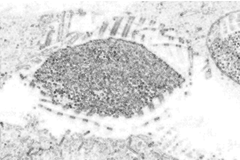
\includegraphics[scale = 0.7]{log_3} & 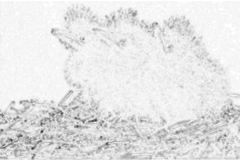
\includegraphics[scale = 0.7]{log_4}\\
\end{tabular}
\caption{Output by brightness gradient segmentation. (Gradient method based on Log).}
\label{table:4}
\end{table}
\end{center}



\begin{center}
\begin{table}
\begin{tabular}{c| c}
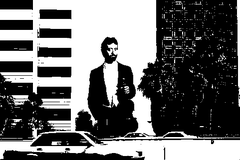
\includegraphics[scale = 0.7]{kmean_1} & 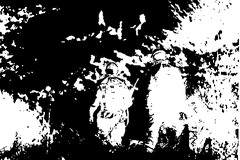
\includegraphics[scale = 0.7]{kmean_2}\\
\\\hline\\
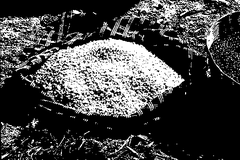
\includegraphics[scale = 0.7]{kmean_3} & 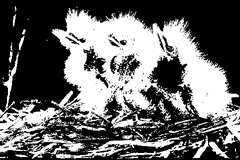
\includegraphics[scale = 0.7]{kmean_4}\\
\end{tabular}
\caption{Output by K-mean Segmentation clustering. (Gradient method based on Log).}
\label{table:4}
\end{table}
\end{center}



\begin{center}
\begin{table}
\begin{tabular}{c| c}
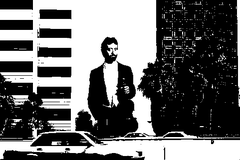
\includegraphics[scale = 0.7]{kmean_1} & 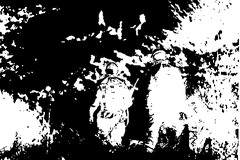
\includegraphics[scale = 0.7]{kmean_2}\\
\\\hline\\
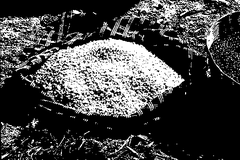
\includegraphics[scale = 0.7]{kmean_3} & 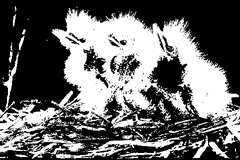
\includegraphics[scale = 0.7]{kmean_4}\\
\end{tabular}
\caption{Output by Mean-shift Segmentation clustering. (Gradient method based on Log).}
\label{table:4}
\end{table}
\end{center}







\section{Methods adopted for Comparing the images}
\section{Result and discussion}
\section{Conclusion}
\end{document}